\pagestyle{fancy}
\vspace*{40 pt}

\subsection{Tela de velocidade}
    Esta tela é responsável por exibir o setpoint atual da máquina e permitir que o operador altere a velocidade da máquina. Para acessar esta tela
    basta clicar no botão de velocidade em qualquer tela. O operador pode selecionar entre as velocidades pré-definidas ou digitar um valor manualmente.
    Para digitar um valor manualmente, basta clicar no campo onde o setpoint é exibido e digitar o valor desejado. Para alterar a velocidade, basta clicar no botão "Confirma",
    para parar a máquina basta clicar no botão "Zerar". Para retornar a tela anterior, basta clicar em qualquer lugar da tela que não seja um botão. Esta tela possui um 
    barra que fornece uma representação visual da velocidade da máquina, quanto mais próxima estiver da cor verde, menor é a velocidade da máquina e quanto mais próxima
    estiver da cor vermelha, mais próximo da velocidade máxima.
    \vspace*{\fill}
    \begin{figure}[h]
      \centering
      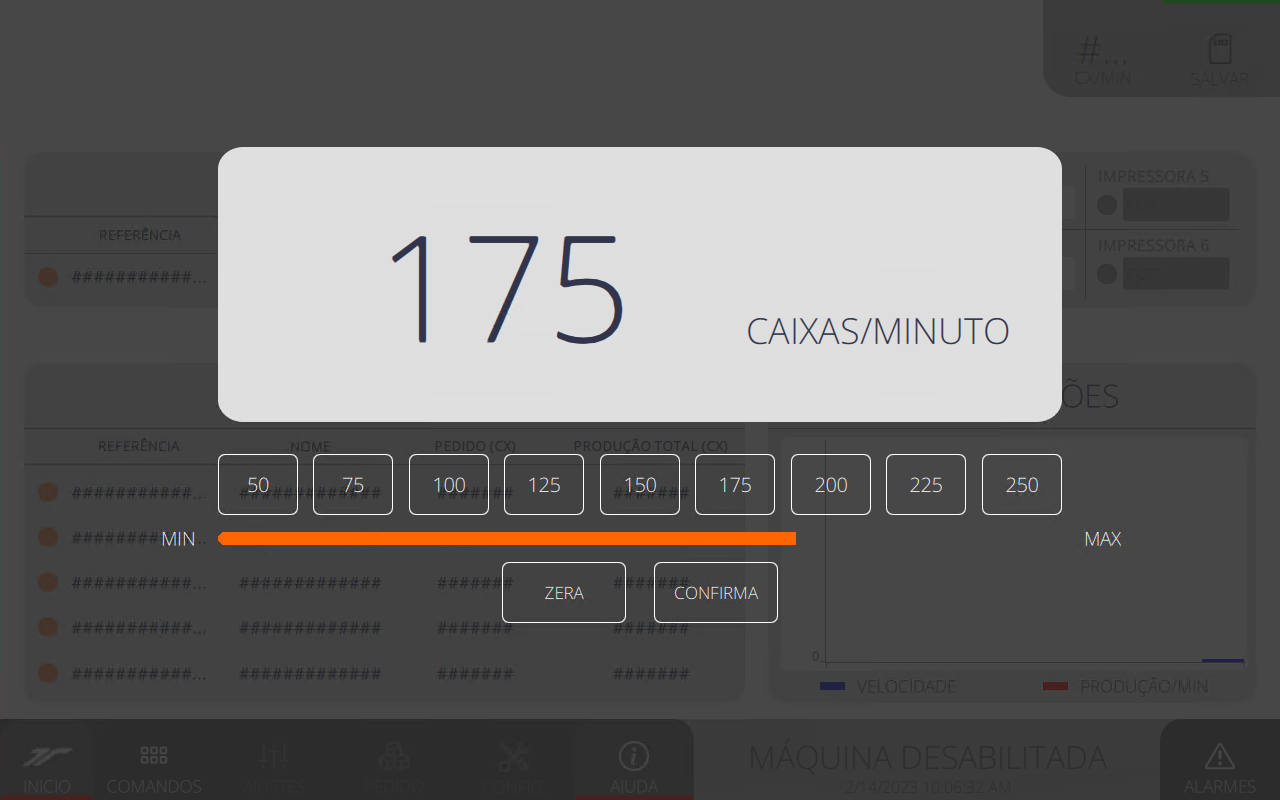
\includegraphics[width=576 px,height=360 px]{src/imagesMiniline/14-speedScreen/1.png}
    \end{figure}
    \vspace*{\fill}
    
    
    